\section{Experiments}
Our main test-bed is an cluster of 6 machines,
each of which is equiped with a 8-core AMD FX-8120 at 3.1 GHz
with 16 GB RAM, running Linux.
A distributed file system (QFS) runs in the cluster manages six 3TB disks
 with default replication degree set to 3.
Our data set consists of 350 virtual machine image snapshots taken from Alibaba.com's
public VM cloud in China. We select 35 VMs from the most popular 7 OSes: 
Debian, Ubuntu, Redhat, CentOS, Win2003 32bit, win2003 64 bit and win2008 64 bit. 
For each OS, 5 VMs are chosen, and every VM come with 10 full snapshots.

\subsection{Replication cost}
\begin{table}
    \begin{tabular}{|c|c|}
    \hline
    PDS replication degree & Total space (GB) \\ \hline
    3                      & 3065             \\ \hline
    4                      & 3072             \\ \hline
    5                      & 3079             \\ \hline
    6                      & 3086             \\ \hline
    7                      & 3093             \\ \hline
    \end{tabular}
\caption{Storage space cost under different PDS replication degree}
\label{tab:replcation_cost}
\end{table}

\subsection{System Performance}
{\bf Single VM Backup} We start the evauluation of our system by examine the normal warmed-up
backup scenario - taking a snapshot of a VM which already has old backups exist. To simulate this
scenario, we pick one 40GB VM from the data set, make an initial snapshot backup, then
evaulate the system performance on the second snapshot backup. We repeat such procedure
under different PDS memory usage settings, the results of backup time break down are shown in
Figure~\ref{fig:single_vm_backup}. 

\begin{figure}
    \centering
    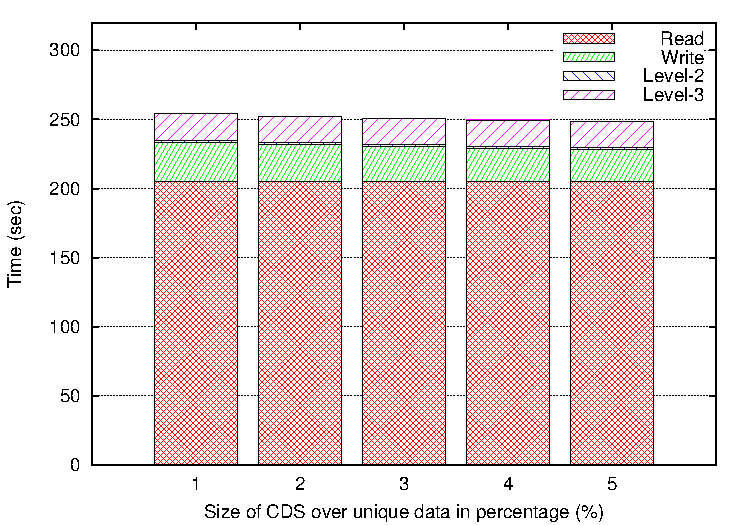
\includegraphics[width=3in]{figures/single_backup_time}
    \caption{Backup times for varying PDS sizes}
    \label{fig:single_vm_backup}
\end{figure}

It's easy to see that the time of I/O dominates the backup process, our deduplication
procedure only takes a tiny fraction of the total backup time. Larger memory permits us to
use larger PDS index to cover more of global index, as a result the amount of data to be writen
is reduced and so do the writing time.
Inside the deduplication procedure, the time costs of level-1
is plainly zero, and the costs of level-2 and level-3 are almost identical under different settings
because the number of fingerprints to process are just the same.

{\bf Parallel VM Backup} We then evaluate the performance of writing snapshots in parallel.
To begin, on each node we let 4 VMs writing snapshot concurrently, and gradually 
increase number of VMs to 12 to saturate our system capability. We observed 
the per-node throughput peaked at 2700 MB/s when writing 10 VM snapshots in parallel, 
which is far beyond our QFS file system capability. The reason behind it is our efficient
deduplication architecture and compression greatly reduce the amount of data that need to be writen to
the file system. The main bottleneck here is our QFS only manages one disk per node, 
making it inefficient to utilize the benefits of parallel disk access. We expect our achitecture can
perform even better in production cluster which normally has more than ten disks on each node.

\begin{figure}
    \centering
    \subfigure[Real VM backup performance]
    {
        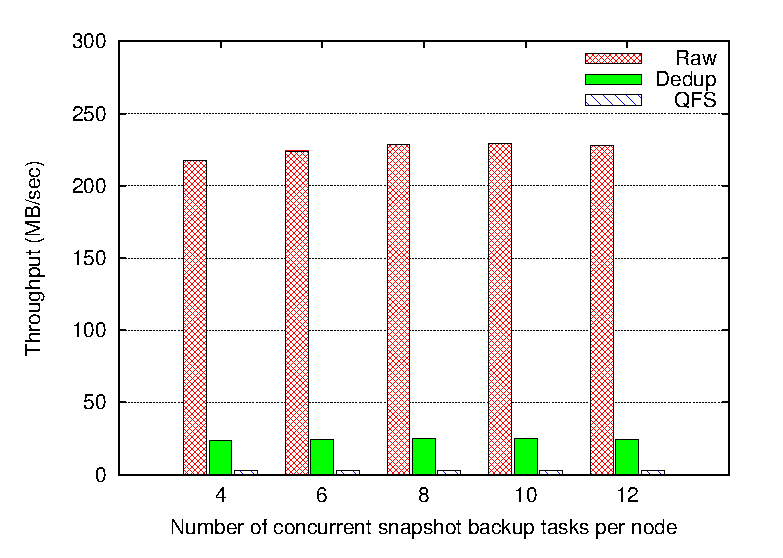
\includegraphics[width=3in]{figures/parallel_backup_with_read}
        \label{fig:withread}
    }
    \\
    \subfigure[Deduplication and storage system performance]
    {
        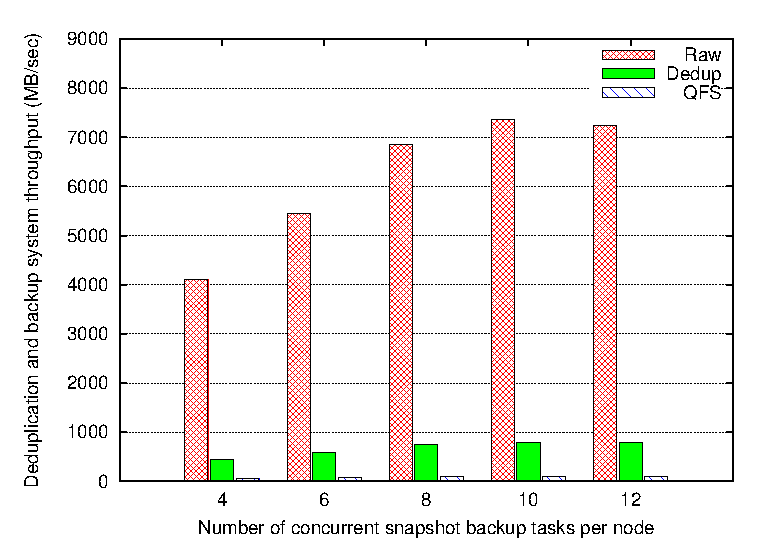
\includegraphics[width=3in]{figures/parallel_backup_no_read}
        \label{fig:noread}
    }
    \caption{Throughput per-node with concurrent snapshot backup tasks}
    \label{fig:parallel_backup}
\end{figure}


% \begin{figure}[htbp]
%   \centering
%   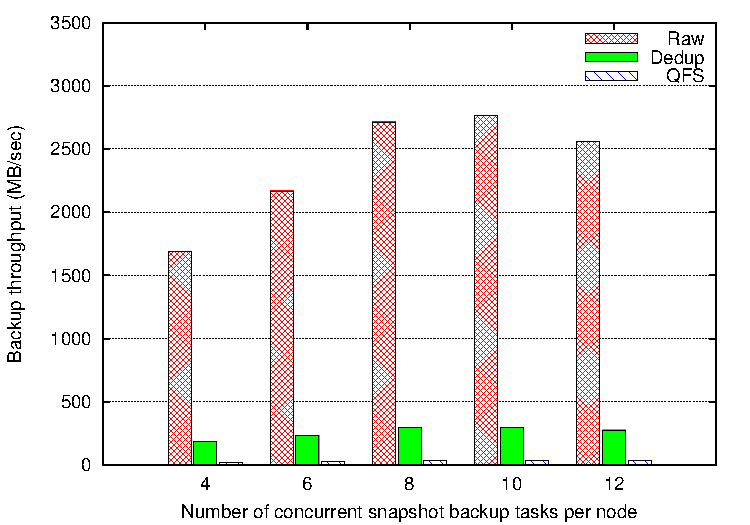
\epsfig{file=figures/parallel_backup, width=3.5in}
%   \caption{Throughput per-node with concurrent snapshot backup tasks}
%   \label{fig:parallel_backup}
% \end{figure}


% \begin{table}
% \begin{tabular}{ |p{1.5cm}|p{1.8cm}|p{1.2cm}|p{1.4cm}| }
% \hline
%  & Costs & Stateless routing with binning (s) & VM-centric approach (s) \\ \hline
% \multirow{4}{*}{\vbox{I/O related}} & Read data & 0.05 & 0.05 \\ \cline{2-4}
%  & Transfer data  & 0.017 & 0.017 \\ \cline{2-4}
%  & Write data & 0.03 & 0.025 \\ \cline{2-4}
%  & Subtotal & 0.097 & 0.092 \\ \hline
% \multirow{5}{*}{\vbox{Dedupe related}} & Read index/recipe & 0.01 & 0.00045 \\ \cline{2-4}
%  & Write index/recipe & 0.01 & 0.0051 \\ \cline{2-4}
%  & Transfer fingerprints & 0.00058 & 0.00013 \\ \cline{2-4}
%  & PDS lookup & N/A & 0.00034 \\ \cline{2-4}
%  & Subtotal & 0.021 & 0.0064 \\ \hline
% \multicolumn{2}{ |c| }{Total} & 0.12 & 0.098 \\
% \hline
% \end{tabular}
% \caption{Time of backup a segment break down}
% \label{tab:compare}
% \end{table}


\subsection{Comparison with Other Approaches}
\subsubsection{Stateless Routing with Binning}
We compare our system with Stateless Routing with Binning (SRB) in terms of
both backup time and deduplication efficiency. SRB is the same as the stateless
routing algorithm given in the Extreme Binning\cite{??} paper. the
deduplication efficiency is compared in
Figure~\ref{fig-exbin-efficiency-graph}, showing the deduplication efficiency
(percent of duplicate chunks which are deduped) of SRB and VC with several
different PDS sizes. From the graph you can see that VC provides similar or
better deduplication efficiency in all cases. In Figure~\ref{fig:srb_vs_vc} you
can see simulated backup times using actual throughput numbers from our test
backup cluster, and VC outperforms SRB mainly due to significantly fewer index
lookups (since SRB uses hash-partitioning, all lookups are essentially random
and caching will be largely innefective).  \emph{Should we use one of the two
bar charts, or the graph? I am thinking the graph, but I'll leave the two bar
charts in the paper until we decide? If we use the bar charts some text will
have to be changed. We could also add each of the PDS sizes to the bar chart
and have 4 bars instead of 2.}
\comments{%both of the bar charts are superceded by the graph below
%\comments{
    %this version of the figure is vertical
    \begin{figure}[ht]
  \centering
    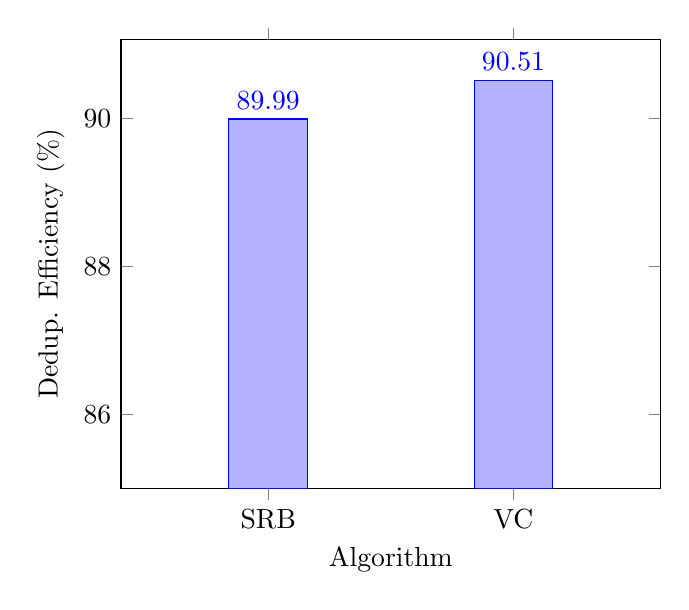
\begin{tikzpicture}
            \begin{axis}[
            %title={Extreme-Binning Efficiency},
            ybar,
            bar width=1.00cm,
            symbolic x coords={SRB,VC},
            xlabel={Algorithm},
            ylabel={Dedup. Efficiency (\%)},
            %extra y ticks={4.5,5.5,6.5} %to add extra ticks
            xtick=data, %without this the symbolic coords may be repeated as filler
            enlarge x limits=0.6, %used to push plots towards center
            ymin=85,
            %ymax=100,
            nodes near coords,
            nodes near coords align={vertical},
            ]
            \addplot coordinates {(SRB,89.99) (VC,90.51)};
            \end{axis}
    \end{tikzpicture}
    \caption{Deduplication Efficiency
        ($efficiency=\frac{d-du}{d-du_{complete}}$) comparison between Stateless Routing with Binning and VC with 2\% PDS.}
  \label{fig-exbin-efficiency1}
\end{figure}
%}
%same figure as above but horizontal (better for only two data points)
\begin{figure}[ht]
  \centering
    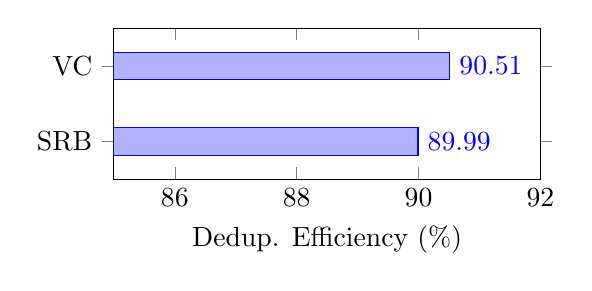
\begin{tikzpicture}
            \begin{axis}[
            %title={Extreme-Binning Efficiency},
            xbar,
            width=7cm,
            height=3.5cm,
            %bar width=0.75cm,
            symbolic y coords={SRB,VC},
            xlabel={Dedup. Efficiency (\%)},
            %ylabel={Algorithm},
            %extra x ticks={4.5,5.5,6.5} %to add extra ticks
            ytick=data, %without this the symbolic coords may be repeated as filler
            enlarge y limits=0.5,
            xmin=85,
            xmax=92, %otherwise label overlaps with right border
            nodes near coords,
            nodes near coords align={horizontal},
            ]
            \addplot coordinates {(89.99,SRB) (90.51,VC)};
            \end{axis}
    \end{tikzpicture}
    \caption{Deduplication Efficiency
        ($efficiency=\frac{d-du}{d-du_{complete}}$) comparison between Stateless Routing with Binning and VC with 2\% PDS.}
  \label{fig-exbin-efficiency2}
\end{figure}
}

%graph comparing extreme binning (SRB) with PDS model (VC) for different cds percentages
\begin{figure}[ht]
  \centering
    \begin{tikzpicture}
            \begin{axis}[
            %title={Ex-Binning Efficiency},
            cycle list name=mline,
            xlabel={Number of VMs added},
            ylabel={Dedup. Efficiency (\%)},
            %extra y ticks={4.5,5.5,6.5} %to add extra ticks
            mark options=solid,
            legend pos=south west,
            %legend columns=2,
            %legend style={
            %    at={(0.5,-0.2)},
            %anchor=north},
            ]
            \addplot table[x=VMs,y=exbin] {figures/exbin_efficiency_comparison.txt};
            \addplot table[x=VMs,y=cds4] {figures/exbin_efficiency_comparison.txt};
            \addplot table[x=VMs,y=cds2] {figures/exbin_efficiency_comparison.txt};
            \addplot table[x=VMs,y=cds1] {figures/exbin_efficiency_comparison.txt};
            \legend{SRB,VC ($\sigma=4\%$),VC ($\sigma=2\%$),VC ($\sigma=1\%$)};
            \end{axis}
    \end{tikzpicture}
    \caption{Deduplication Efficiency
        ($efficiency=\frac{d-du}{d-du_{complete}}$) comparison between
    Stateless Routing with Binning and VC.}
  \label{fig-exbin-efficiency-graph}
\end{figure}

\begin{figure}[htbp]
  \centering
  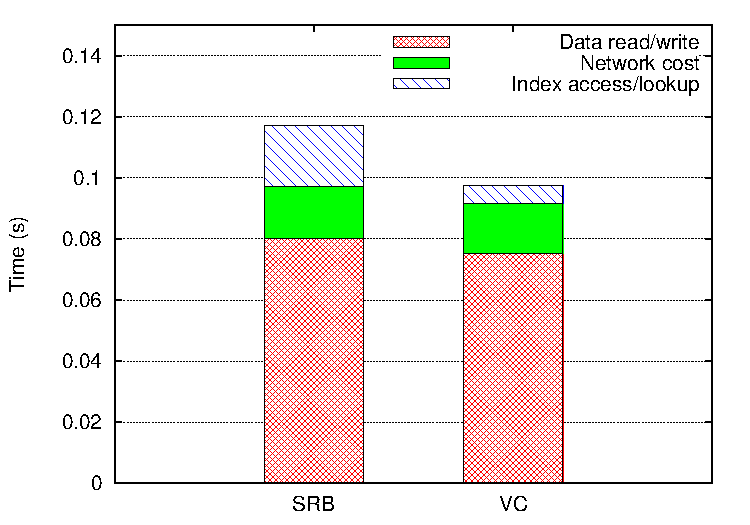
\epsfig{file=figures/srb_vs_vc, width=3.5in}
  \caption{Time to backup a dirty segment under SRB and VC approach}
  \label{fig:srb_vs_vc}
\end{figure}

\comments{
\subsection{Read Snapshot}

\subsection{Comparison with Other Approaches}
\subsubsection{Sampled Index}
One alternative approach to avoiding a single global index is to use a sampled
index. This is the approach taken by Guo and Efstathopoulos\cite{Guo2011}. We
compare their solution to ours by running their algorithm on our 350 traces
using a sampling rate of 1 out of 101 blocks, and always including the first
block in a container (which we fix at 16MB in size). The results of running this
test are shown in Table~\ref{??}, and the memory usage comparison can be found
Sec.~\ref{??}. Our results show that using a sampled index achieves a very high
rate of deduplication, and so a sampled index might be a good way to do dedup
in a single node setup.

The problems for sampling are in distributing the
algorithm and in deduplicating extremely large bodies of data. The algorithm
stores the entire (sampled) index in memory, which is required for high
throughput to avoid the disk-bottleneck problem - since the index itself has no
locality information, lookups are essentially random, so the index must be
somehow optimized to prevent excessive disk seeking (the sampling algorithm does
this by storing the index in memory). To distribute this index, each node would
either require a complete copy of the index which would have a prohibitive cost in
memory, or something like memcached must be used, which leaves the same problem
as the disk bottleneck with every index check potentially using the network.
The difficulty in storing extremely large bodies of data
is related, as once 1PB is stored in the system, assuming a sampling rate of 
1/101 with 22 byte index entires, 55GB of (in memory) index are required.

Our solution uses more total memory (??how much??), but is more scalable both in
terms of capactity and distributing the deduplication. The only part of our
algorithm which requires significant network traffic is the PDS deduplication,
but this is done after Levels 1 and 2 (dirty bits and comparison to parent), and
so is only done for a small percent of blocks (?? 5-10\% ??).

\subsubsection{Scalable Data Routing}
Another approach to avoiding a global index is to use a content-based hash
partitioning algorithm to break up the deduplication work. This approach is
taken by Dong et al. in their Scalable Data Routing paper, and is similar to
Exreme Binning\cite{??}\cite{extreme_binning09}. We compared our solution to
content-based hash partitioning by running the algorithm on our set of 
traces. We used 2MB superchunks and 4KB chunks to partition the data, and use
the minhashes of the superchunks for routing. The results of this are shown in
Table~\ref{??}. Routing each chunk to a bin provides good deduplication
efficiency, and only requires each storage node to keep an index of local data
and the bin mapping, but misses significant opportunities in our indended use
case.

The problem with the Data Routing algorithm is in the very high network traffic.
Our intended use case is a backup system which runs alongside a number of VMs,
in order to save costs. Data Routing makes no use of the inherent locality in
such a system, and therefore puts a much higher network burden on machines which
are also running 35 VMs each. This will reduce the available network bandwidth
to users of the VMs, and/or reduce the possible deduplication throughput.

}
